\documentclass[12pt,a4paper]{article}
\usepackage[utf8]{inputenc}
\usepackage{amsmath}
\usepackage{amsfonts}
\usepackage{listings}
\usepackage{graphicx}
\usepackage{geometry}
\geometry{margin=1in}
\usepackage{hyperref}
\hypersetup{
    colorlinks=true,
    linkcolor=blue,
    urlcolor=blue
}
\usepackage{setspace}
\setstretch{1.2}

\title{\textbf{Regex to NFA}}
\author{Darth-218}
\date{}

\lstset{
    basicstyle=\ttfamily\footnotesize,
    backgroundcolor=\color[gray]{0.95},
    frame=single,
    breaklines=true
}

\begin{document}

\maketitle

\section*{Installation and Running}

To install the required dependencies and run the project:

\begin{lstlisting}[language=bash]
pip install -r requirements.txt

streamlit run main.py   # For the GUI
python cli.py           # For the CLI
\end{lstlisting}

\section*{Project Components}

\begin{itemize}
    \item Parser
    \item NFA Constructor
    \item NFA Visualizer
\end{itemize}

\section*{Valid Regex Operators}

\begin{itemize}
    \item \texttt{.}: Concatenation (concat)
    \item \texttt{|}: Union (union)
    \item \texttt{*}: Kleene star (star)
    \item \texttt{+}: Kleene plus (plus)
    \item \texttt{?}: Optional (optional)
\end{itemize}

\section*{Parsing}

\textbf{Goal:} Convert an input string regex into a structured blueprint for representation.

\textbf{Input:} A valid string regex.\\
\textbf{Output:} Abstract syntax tree (AST).

\subsection*{Parser Grammar}

\[
\begin{aligned}
\text{Expression} &\rightarrow \text{Term} + \text{Term} \mid \text{Term} \\
\text{Term} &\rightarrow \text{Factor} \cdot \text{Character} \mid \text{Factor} \\
\text{Factor} &\rightarrow \text{Base} \mid \text{Operation} \\
\text{Base} &\rightarrow (\text{Expression}) \mid \text{Character} \\
\text{Operation} &\rightarrow * \mid ? \mid +
\end{aligned}
\]

\subsection*{Example AST}

For the regex \texttt{(a|b)*abb}:

\begin{lstlisting}[language=Python]
ast_representation = {
    "type": "concat",
    "left": {
        "type": "star",
        "left": {
            "type": "union",
            "left": "a",
            "right": "b"
        },
        "right": 0, # kleene star is a unary operator
    },
    "right": {
        "type": "concat",
        "left": "a",
        "right": {
            "type": "concat",
            "left": "b",
            "right": "b"
        }
    }
}
\end{lstlisting}

\section*{Constructing}

\textbf{Goal:} Convert the blueprint into an actual NFA.\\
\textbf{Input:} AST.\\
\textbf{Output:} Data representing NFA (Formal definition).

\subsection*{Process}

Handle operations using Thompson's Construction Algorithm.

\subsection*{Example NFA}

For the regex \texttt{(a|b)*abb}:

\begin{lstlisting}[language=Python]
nfa_representation = {
    "states": {0, 1, 2, 3, 4, 5, 6, 7, 8, 9, 10, 11},
    "start_state": 0,
    "accept_states": {11},
    "transitions": {
        0: {"_e": {1, 7}}, # _e is used as epsilon.
        1: {"a": {2}},
        2: {"_e": {6}},
        7: {"b": {8}},
        8: {"_e": {6}},
        6: {"_e": {0, 9}},
        9: {"a": {10}},
        10: {"b": {11}},
        11: {"b": {12}}
    }
}
\end{lstlisting}

\section*{Visualization}

\textbf{Goal:} Visualize the NFA.\\
\textbf{Input:} NFA representation.\\
\textbf{Output:} NFA graph.

\subsection*{Process}

\begin{enumerate}
    \item Input text field to enter the regex.
    \item ``Visualize'' button.
    \item A box to show the output NFA.
\end{enumerate}

\subsection*{Example Visualization}

For the regex \texttt{(a|b)*abb}:

\begin{center}
    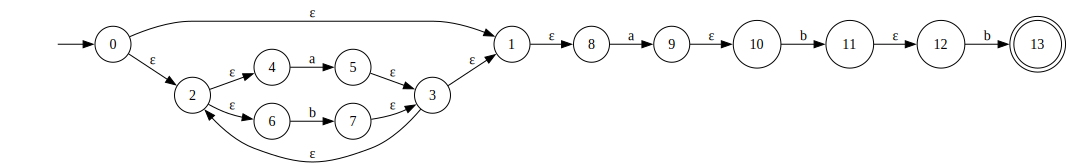
\includegraphics[width=0.7\textwidth]{example.svg}
\end{center}

\end{document}
